\documentclass[
10pt,
a4paper,
oneside,
headinclude,footinclude, 
BCOR5mm,
]{scrartcl}

\usepackage{pgf}
\usepackage{tikz}
\usetikzlibrary{arrows,automata}
\definecolor{dgreen}{HTML}{00994C}

\input{structure.tex}

\hyphenation{Fortran hy-phen-ation}

\title{\normalfont\spacedallcaps{Automata \& Computability}}
\author{\spacedlowsmallcaps{Jensen Bernard}}
\date{}

\begin{document}

\renewcommand{\sectionmark}[1]{\markright{\spacedlowsmallcaps{#1}}}
\lehead{\mbox{\llap{\small\thepage\kern1em\color{halfgray} \vline}\color{halfgray}\hspace{0.5em}\rightmark\hfil}}
\pagestyle{scrheadings}

\maketitle

\setcounter{tocdepth}{1} % Contents table depth

\tableofcontents

\section*{Abstract} 

Dit document is tot stand gekomen om een hulp te zijn bij het studeren van het vak \textbf{Automaten en Berekenbaarheid}. Het bevat enkel voorbeelden van examenvragen, samen met een uitgewerkte oplossing. In geen enkel geval kan dit document de cursus vervangen. Ik raad aan om de cursus, die verkrijgbaar is via de cursusdienst van \textbf{Scientica}, eerst door te nemen om op zijn minst te weten waarover het gaat. Indien u fouten vindt of informatie wil toevoegen, kan dit altijd via Github. Good luck*.

{\let\thefootnote\relax\footnotetext{* \textit{You'll need it.}}}

\newpage 

\section{Voorwoord}

\lipsum[1-3]

\section{Talen en Automaten}

\lipsum[5] 

\section{Talen en Berekenbaarheid}

\subsection{$A_{TM}$ is niet-beslisbaar}

\textbf{Bewijs in detail dat $A_{TM}$ niet beslisbaar is en steun daarbij niet op de stelling van Rice. Zou het helpen als het toegelaten was op de stelling van Rice te steunen? Is $A_{TM}$ herkenbaar? Co-herkenbaar?}

\vspace{5mm}
\textbf{$A_{TM}$ is niet beslisbaar}
\begin{proof}
	Beter bekend als het acceptatieprobleem voor Turingmachines. De geassocieerde taal is 
	\begin{center}
	$A_{TM} = \{ <M,s> |$ \textit{$M$ is een Turingmachine en} $ s \in L_M\}$
	\end{center}
	Stel er bestaat een beslisser $B$ voor $A_{TM}$. Dat betekent dat bij input $<M,s>$ $B$ accepteert als $M$ bij input $s$ stopt in zijn $q_a$ en verwerpt als $M$ bij input $s$ stopt in zijn $q_r$ of loopt. We schrijven
	\begin{center}
		$B(<M,s>)$ \textit{is accept als $M$ $s$ accepteert en anders reject}
	\end{center}
	Construeer nu de contradictie machine $C$ met eigenschap:
	\begin{center}
		$C(<M>) = opposite(B(<M,M>))$ \textit{voor elke Turingmachine $M$}
	\end{center}
	Daarbij is $opposite(accept) = reject$ en $opposite(reject) = accept$. \\
	Neem nu voor $M$ hierboven $C$ zelf, dan krijgen we:
	\begin{center}
		$C(<C>) = opposite(B(<C,C>))$
	\end{center}		
	Als $C(<C>) = accept$, dan is $B(<C,C>) = accept$, dan is $opposite(B(<C,C>)) = reject$, dan is $C(<C>) = reject$, dan is $B(<C,C>) = reject$, dan is $opposite(B(<C,C>)) = accept$, dan is $C(<C>) = accept$ \dots \\
	Dus $C$ kan niet bestaan, dus $B$ bestaat niet. Dus $A_{TM}$ is niet beslisbaar.
\end{proof} 

\textbf{$A_{TM}$ is herkenbaar}
\begin{proof}
	De herkenner $A$ voor $A_{TM}$ laat, met input $<M,x>$, $M$ lopen op $s$. Indien deze $M$ $s$ accepteerd, dan accepteerd $A$ zijn input. Indien deze de input $reject$, of gewoon niet stopt, dan zal $A$ deze ook niet accepteren. $A_{TM}$ is dus herkenbaar.
\end{proof}

\textbf{$A_{TM}$ is niet co-herkenbaar}
\begin{proof}
	$A_{TM}$ kan echter niet co-herkenbaar zijn. We bewijzen dit met contradictie. Indien $A_{TM}$ co-herkenbaar is, is deze dus herkenbaar en co-herkenbaar (zie vorig bewijs). Wanneer een taal deze beide eigenschappen bezit, is deze beslisbaar. Dit is een contradictie met het eerste bewijs.
\end{proof}

\textbf{De stelling van Rice} \vspace{-1mm} \\ \\
Deze stelling bewijst dat elke taal (die aan bepaalde voorwaarden voldoet) niet-beslisbaar is. Hier gaan we zo dadelijk dieper op in. We moeten eerst de volgende twee definities toelichten alvorens we verder kunnen gaan met het bewijs van $A_{TM}$, gebruik makend van deze stelling (wat korter zal zijn dan voorgaande bewijzen).

\begin{theorem}[De niet-triviale eigenschap]
	Een eigenschap $P$ van Turingmachines heet niet-triviaal indien $Pos_P \neq \emptyset$ en ook $Neg_p \neq \emptyset$.
\end{theorem}

\begin{theorem}[Taal-invariante eigenschap]
	Een eigenschap $P$ heet taal-invariant indien alle machines die dezelfde taal bepalen, hebben ofwel allemaal $P$, ofwel heeft geen enkele ervan $P$. \\
	 $$L_{M_1} = L_{M_2} \Rightarrow P(M_1) = P(M_2)$$
\end{theorem}

\begin{theorem}[Formelere stelling van Rice]
	Voor elke niet-triviale, taal-invariante eigenschap $P$ van Turingmachines geldt dat $Pos_P$ (en ook $Neg_P$) niet beslisbaar is.
\end{theorem}

\begin{proof}
	Veronderstel dat $M_\emptyset$ (de machine die de lege taal beslist) de eigenschap $P$ niet heeft - indien dat niet zo is, verander dan $P$ in zijn negatie. Vermits $P$ niet-triviaal is, bestaat er een taal $L_X$ zodat $X$ een Turingmachine is met de eigenschap $P$. Stel dat $Pos_P$ (en dus ook $Neg_P$) beslisbaar id: we zullen een beslisser $B$ voor $Pos_P$ gebruiken om een beslisser $A$ te maken voor $A_{TM}$. $A$ krijgt als input $<M,s>$ en doet het volgende:
	\begin{enumerate}
		\item construeer een hulpmachine $H_{M,s}$ die het volgende doet bij input $x$:
		\begin{enumerate}
			\item laat $M$ lopen op $s$
			\item indien $M$ $s$ accepteert, laat dan $X$ lopen op $x$ en accepteer als $X$ $x$ accepteert
		\end{enumerate}
		\item laat nu $B$ los op $H_{M,s}$
		\item als $B$ $H_{M,s}$ accepteert, dan $accept$, anders $reject$
	\end{enumerate}
	$H_{M,s}$ accepteert ofwel de lege taal, ofwel $L_X$ (TODO: waarom).\\
	\begin{center}
		$A$ \textit{accepteert} $<M,s>$ \\
		$\Updownarrow$ \\
		$B$ $H_{M,s}$ \textit{accepteert} \\
		$\Updownarrow$ \\
		$H_{M,s}$ \textit{de eigenschap} $P$ \textit{heeft} \\
		$\Updownarrow$ \\
		$H_{M,s}$ \textit{accepteert} $L_X$ \\
		$\Updownarrow$ \\
		$M$ \textit{accepteert} $s$
	\end{center}
	Dus, $A$ is een beslisser voor $A_{TM}$, hetgeen niet kan, dus kan $B$ niet bestaan en $Pos_P$ is niet beslisbaar.
\end{proof}

\newpage
\subsection{Reduceerbaarheid}

\textbf{Bespreek de twee noties van reduceerbaarheid ($A \leq_m B$ en $A \leq_T B$), hun verband en op welke manier die noties kunnen gebruikt worden om aan te tonen dat een taal (on)beslisbaar/herkenbaar is.}

\vspace{5mm}
\textbf{Veel-\'e\'en reductie} \vspace{-4mm} \\ \\

\noindent Om over te gaan naar de definitie van de reductie van talen, kunnen we best eerst de definifie van Turing-berekenbaar erbij halen (indien we dit niet doen, kunnen we zeker zijn van deze bijvraag).

\begin{theorem}[Turing-berekenbare functie]
	Een functie $f$ heet Turing-berekenbaar indien er een Turingmachine bestaat die bij input $s$ uiteindelijk stopt met $f(s)$ op de band.
\end{theorem}

\begin{theorem}
	We zeggen dat taal $L_1$ (over $\Sigma_1$) naar taal $L_2$ (over $\Sigma_2$) kan gereduceerd worden indien er een afbeelding $f$ met signatuur $\Sigma^*_1\longrightarrow \Sigma^*_2$ bestaat zodanig dat $f(L_1) \subseteq L_2$ en $f(\overline{L_1}) \subseteq \overline{L_2}$, en zodanig dat $f$ Turing-berekenbaar is. We noteren dat door $L_1 \leq_m L_2$.
\end{theorem}

\newpage
\section{Herschrijfsystemen}

\lipsum[4-5]

\section{Andere Rekenparadigma's}

\lipsum[10]

\section{Talen en Complexiteit}

\lipsum[11]

\newpage
\section{Bewijzen onder de loop}

\subsection{Overzicht}

\noindent In dit hoofdstuk zullen bewijzen verder uitgelegd (of vereenvoudigd) worden. Deze bewijzen worden gebruikt in de oplossingen van de examens, maar zijn soms moeilijk te begrijpen.\\

\noindent De modeloplossingen die doorheen dit document werden beschreven, bevatten soms moeilijke en complexe bewijzen. Dit hoofdstuk is bedoeld om deze volledig te beheersen. Probeer wel de vorige notaties te gebruiken voor het examen, aangezien dit de structuur is die de professor zelf gebruikt. Dit hoofdstuk is enkel ter verduidelijking.

\subsection{De stelling van Rice}

\noindent Om de stelling van Rice te bewijzen, is het best dat we eerst even twee definities uit de cursus herhalen, namelijk deze van de niet-triviale eigenschap en deze van de taal-invariante eigenschap.

\begin{theorem}[Niet-triviale eigenschap]
	Een eigenschap $P$ van Turingmachines heet niet-triviaal indien $Pos_p \neq \emptyset$ en ook $Neg_p \neq \emptyset$. Er bestaan dus Turingmachines die deze eigenschap $P$ bezitten, maar ook machines die deze niet bezitten.
\end{theorem}

\begin{theorem} [Taal-invariante eigenschap]
	De eigenschap $P$ heet taal-invariant indien alle machines die dezelfde taal bepalen hebben ofwel allemaal $P$, ofwel heeft geen enkele ervan $P$.
	$$L_{M_1} = L_{M_2} \Rightarrow P(M_1) = P(M_2)$$
\end{theorem}

\noindent Met deze twee definities in het achterhoofd, kunnen we overgaan naar de formele definitie van de stelling van Rice, met het bewijs als gevolg.

\begin{theorem}[Stelling van Rice]
	Voor elke niet-triviale, taal-invariante eigenschap $P$ van Turingmachines geldt dat $Pos_P$ (en ook $Neg_P$) niet beslisbaar is.
\end{theorem}

\begin{proof}
	Neem aan dat de Turingmachine $M_\emptyset$ de lege taal beslist. Laten we er nu van uit gaan dat deze machine een bepaalde eigenschap $P$ heeft. De stelling zegt ons dat de eigenschap $P$ niet-triviaal is. Uit de definitie kunnen we dan afleiden dat $Pos_P \neq \emptyset$ (en ook $Neg_P \neq \emptyset$). Aangezien deze verzameling niet leeg is, moet er een Turingmachine $X$ bestaan met deze eigenschap $P$. Laat ons zeggen dat deze Turingmachine de taal $L_X$ beslist.\\\\
	We gaan nu proberen een contradictie te bekomen door aan te nemen dat de stelling niet waar is. We nemen dus aan dat $Pos_P$ (en dus ook $Neg_P$) beslisbaar is. We gaan nu een beslisser $B$ proberen op te stellen voor $Pos_P$ die deze beslist\footnote{Later zullen we deze $B$ gebruiken om een beslisser $A$ te maken voor $A_{TM}$}. Om $B$ te maken, gaan we eerst een hulpmachine $H_{M,s}$ opstellen.\\\\
	Deze hulpmachine $H_{M,s}$ heeft een Turingmachine $M$ en een string $s$ in zich. Deze staan vast voor de machine en kunnen dus niet veranderen\footnote{Ze zijn als het ware gehardcoded.}. De input van deze machine is een string $x \in L_X$. Wanneer $H_{M,s}$ gestart wordt, zal deze eerst $M$ laten lopen over $s$. Indien $M$ $s$ reject, zal $H_{M,x}$ \textbf{altijd} rejecten. Indien $M$ $s$ accept, dan zal $H_{M,s}$ overgaan naar fase 2. Hier zal de hulpmachine $X$ over $x$ laten lopen. Indien $X$ $x$ ook accept, dan zal de hulpmachine accepten. Indien $X$ $x$ reject, dan zal ook de hulpmachine rejecten.\\
	Er zijn nu twee mogelijkheden voor $H_{M,s}$. Indien $M$ $s$ accept, dan gaat $H_{M,s}$ \textbf{altijd} overgaan tot het testen van $x$ in $X$. In dit geval beslist $H_{M,s}$ de volledige taal $L_X$. De andere optie is dat $M$ $s$ reject. In dat geval gaat de hulpmachine \textbf{altijd} rejecten en dus enkel de lege taal accepteren.\\\
	Laat nu de beslisser $B$ los op $H_{M,s}$. Dit wil zeggen dat de beslisser accept of reject voor de gegeven $M$ en $s$.\\
	
\begin{figure}[h!]
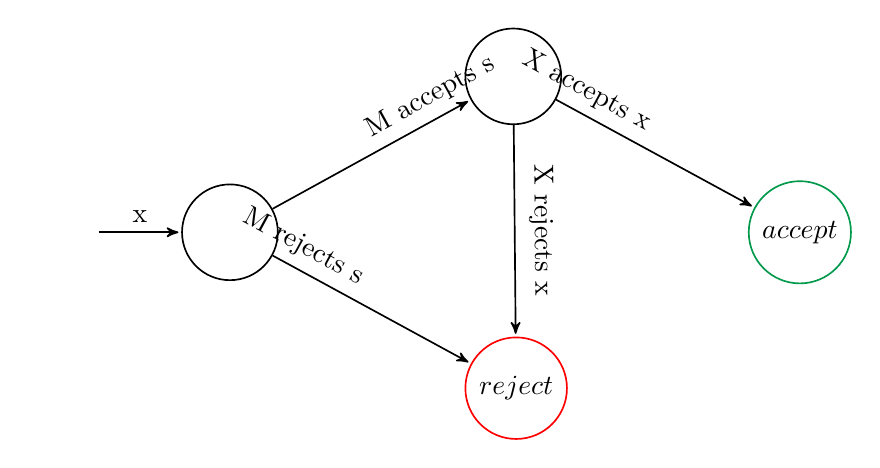
\begin{tikzpicture}[->,>=stealth',shorten >=1pt,auto,node distance=2.8cm,
                    semithick]
  %\tikzstyle{every state}=[fill=red,draw=none,text=white]

  \node[state, color=white] (empty) {};
  \node[state, right of=empty, right=-13mm, inner sep=4.3mm] (A) {};
  \node[state] (B) [above right of=A, right=10mm, inner sep=4.3mm] {};
  \node[state] (D) [below right of=A, right=10mm, draw=red] {$reject$};
  \node[state] (C) [below right of=B, right=10mm, draw=dgreen] {$accept$};

  \path (empty) edge node {x} (A)
  			(A) edge node [sloped, pos=0.85] {M accepts s} (B)
  			(A) edge node [sloped, pos=0.1] {M rejects s} (D)
  			(B) edge node [sloped, pos=0.5, above=0.6mm] {X rejects x} (D)
  			(B) edge node [sloped, pos=0.1] {X accepts x} (C)
;
\end{tikzpicture}
\caption{Visuele voorstelling van de hulpmachine $H_{M,s}$}
\end{figure}
	Stel dat we nu een beslisser $A$ maken voor $A_{TM}$. In dat geval moeten we dus elke $M$ en $s$ in $A_{TM}$ testen. We kunnen dus zeggen dat $A$ accept indien $B$ $H_{M,s}$ accept, anders reject. We bekomen dus de volgende conclusie.
	\begin{center}
		$A$ accepts $<M,s>$\\
		$\Updownarrow$\\
		$B$ accepts $H_{M,s}$\\
		$\Updownarrow$\\
		$H_{M,s}$ heeft eigenschap $P$\\
		$\Updownarrow$\\
		$H_{M,s}$ accepts $L_X$\\
		$\Updownarrow$\\
		$M$ accepts $s$
	\end{center}
	Conclusie: $A$ is een beslisser voor $A_{TM}$, maar dit is onmogelijk aangezien $A_{TM}$ niet beslisbaar is! Hieruit kunnen we concluderen dat $B$ niet bestaat en dus is $Pos_P$ niet beslisbaar. \textbf{Contradictie}.
\end{proof}



\renewcommand{\refname}{\spacedlowsmallcaps{References}}

\bibliographystyle{unsrt}

\bibliography{sample.bib}

\end{document}